% !TEX TS-program = xelatex
% !BIB program = bibtex
% !TeX spellcheck = ru_RU
% !TEX root = talk.tex

\documentclass
  [ russian
  , aspectratio=1610 % Для защит онлайн лучше использовать разрешение не 4х3
  ] {beamer}


% !TeX spellcheck = ru_RU
% !TEX root = vkr.tex
% Опциональные добавления используемых пакетов. Вполне может быть, что они вам не понадобятся, но в шаблоне приведены примеры их использования.
\usepackage{tikz} % Мощный пакет для создание рисунков, однако может очень сильно замедлять компиляцию
\usetikzlibrary{decorations.pathreplacing,calc,shapes,positioning,tikzmark}

% Библиотека для TikZ, которая генерирует отдельные файлы для каждого рисунка
% Позволяет ускорить компиляцию, однако имеет свои ограничения
% Например, ломает пример выделения кода в листинге из шаблона
% \usetikzlibrary{external}
% \tikzexternalize[prefix=figures/]

\newcounter{tmkcount}

\tikzset{
    use tikzmark/.style={
            remember picture,
            overlay,
            execute at end picture={
                    \stepcounter{tmkcount}
                },
        },
    tikzmark suffix={-\thetmkcount}
}

\usepackage{booktabs} % Пакет для верстки "более книжных" таблиц, вполне годится для оформления результатов
% В шаблоне есть команда \multirowcell, которой нужен этот пакет.
\usepackage{multirow}
\usepackage{siunitx} % для таблиц с единицами измерений

% Для названий стоит использовать \textsc{}
\newcommand{\dollar}{\mbox{\textdollar}}
\newcommand{\OCaml}{\textsc{OCaml}}
\newcommand{\C}{\textsc{C}}
\newcommand{\miniKanren}{\textsc{miniKanren}}
\newcommand{\BibTeX}{\textsc{BibTeX}}
\newcommand{\vsharp}{\textsc{V$\sharp$}}
\newcommand{\fsharp}{\textsc{F$\sharp$}}
\newcommand{\csharp}{\textsc{C\#}}
\newcommand{\GitHub}{\textsc{GitHub}}
\newcommand{\SMT}{\textsc{SMT}}

\definecolor{eclipseGreen}{RGB}{63,127,95}
% \lstdefinelanguage{ocaml}{
% keywords={@type, function, fun, let, in, match, with, when, class, type,
% nonrec, object, method, of, rec, repeat, until, while, not, do, done, as, val, inherit, and,
% new, module, sig, deriving, datatype, struct, if, then, else, open, private, virtual, include, success, failure,
% lazy, assert, true, false, end},
% sensitive=true,
% commentstyle=\small\itshape\ttfamily,
% keywordstyle=\ttfamily\bfseries, %\underbar,
% identifierstyle=\ttfamily,
% basewidth={0.5em,0.5em},
% columns=fixed,
% fontadjust=true,
% literate={->}{{$\to$}}3 {===}{{$\equiv$}}1 {=/=}{{$\not\equiv$}}1 {|>}{{$\triangleright$}}3 {\\/}{{$\vee$}}2 {/\\}{{$\wedge$}}2 {>=}{{$\ge$}}1 {<=}{{$\le$}} 1,
% morecomment=[s]{(*}{*)}
% }

\makeatletter
\@ifclassloaded{beamer}{
    %%% Обязательные пакеты
    %% Beamer
    \usepackage{beamerthemesplit}
    \usetheme{SPbGU}
    \beamertemplatenavigationsymbolsempty
    \usepackage{appendixnumberbeamer}

    %% Локализация
    \usepackage{fontspec}
    \setmainfont{CMU Serif}
    \setsansfont{CMU Sans Serif}
    \setmonofont{CMU Typewriter Text}
    %\setmonofont{Fira Code}[Contextuals=Alternate,Scale=0.9]
    %\setmonofont{Inconsolata}
    \usepackage{polyglossia}
    \setmainlanguage{russian}
    \setotherlanguage{english}

    %% Графика
    \usepackage{pdfpages} % Позволяет вставлять многостраничные pdf документы в текст

    % Математические окружения с русским названием
    \newtheorem{rutheorem}{Теорема}
    \newtheorem{ruproof}{Доказательство}
    \newtheorem{rudefinition}{Определение}
    \newtheorem{rulemma}{Лемма}
    \usepackage{fancyvrb}
}
{}
\makeatother

\usepackage[autostyle]{csquotes} % Правильные кавычки в зависимости от языка
\usepackage{totcount}
\usepackage{setspace}
\usepackage{amsmath, amsfonts, amssymb, amsthm, mathtools} % "Адекватная" работа с математикой в LaTeX

\makeatletter

%!TEX root = vkr.tex

%% Параметры заполнения титульного листа
\usepackage{xkeyval}

%% Русскоязычный вариант
\define@key[ru]{mytitle}{chair}{\def\my@title@chair@ru{#1}}
\define@key[ru]{mytitle}{title}{\def\my@title@title@ru{#1}}
\define@key[ru]{mytitle}{group}{\def\my@title@group@ru{#1}}
\define@key[ru]{mytitle}{author}{\def\my@title@author@ru{#1}}
\define@key[ru]{mytitle}{supervisor}{\def\my@title@supervisor@ru{#1}}
\define@key[ru]{mytitle}{supervisorPosition}{\def\my@title@supervisorPosition@ru{#1}}
\define@key[ru]{mytitle}{reviewer}{\def\my@title@reviewer@ru{#1}}
\define@key[ru]{mytitle}{reviewerPosition}{\def\my@title@reviewerPosition@ru{#1}}
\define@key[ru]{mytitle}{consultant}{\def\my@title@consultant@ru{#1}}
\define@key[ru]{mytitle}{consultantPosition}{\def\my@title@consultantPosition@ru{#1}}
\define@key[ru]{mytitle}{year}{\def\my@title@year@ru{#1}}
\define@key[ru]{mytitle}{specialty}{\def\my@title@specialty@ru{#1}}
\define@key[ru]{mytitle}{programme}{\def\my@title@programme@ru{#1}}
\define@key[ru]{mytitle}{profile}{\def\my@title@profile@ru{#1}}
\define@choicekey*[ru]{mytitle}{type}{coursework,practice,prediploma,master,bachelor,production}{\def\my@title@type@ru{#1}}
\define@choicekey*[ru]{mytitle}{kind}{solution,experiment,production,comparison,theoretical}{\def\my@title@kind@ru{#1}}

%% Англоязычный вариант
\define@key[en]{mytitle}{chair}{\def\my@title@chair@en{#1}}
\define@key[en]{mytitle}{title}{\def\my@title@title@en{#1}}
\define@key[en]{mytitle}{group}{\def\my@title@group@en{#1}}
\define@key[en]{mytitle}{author}{\def\my@title@author@en{#1}}
\define@key[en]{mytitle}{supervisor}{\def\my@title@supervisor@en{#1}}
\define@key[en]{mytitle}{supervisorPosition}{\def\my@title@supervisorPosition@en{#1}}
\define@key[en]{mytitle}{reviewer}{\def\my@title@reviewer@en{#1}}
\define@key[en]{mytitle}{reviewerPosition}{\def\my@title@reviewerPosition@en{#1}}
\define@key[en]{mytitle}{consultant}{\def\my@title@consultant@en{#1}}
\define@key[en]{mytitle}{consultantPosition}{\def\my@title@consultantPosition@en{#1}}
\define@key[en]{mytitle}{year}{\def\my@title@year@en{#1}}
\define@key[en]{mytitle}{specialty}{\def\my@title@specialty@en{#1}}
\define@key[en]{mytitle}{programme}{\def\my@title@programme@en{#1}}
\define@key[en]{mytitle}{profile}{\def\my@title@profile@en{#1}}
\define@choicekey*[en]{mytitle}{type}{coursework,practice,prediploma,master,bachelor}{\def\my@title@type@en{#1}}
\define@choicekey*[en]{mytitle}{kind}{solution,experiment,production,comparison,theoretical}{\def\my@title@kind@en{#1}}

\newcommand{\filltitle}[2]{
    %% Значения по умолчанию для обоих языков
    \ifthenelse{\equal{#1}{ru}}
    {
        \presetkeys[#1]{mytitle}{
            year = {\the\year},
            type = {practice},
            reviewer = {},
            consultant = {},
            profile = {}
        }{}
    }
    {}
    \ifthenelse{\equal{#1}{en}}
    {
        \presetkeys[#1]{mytitle}{
            year = {\the\year},
            type = {practice},
            reviewer = {},
            consultant = {},
            profile = {}
        }{}
    }
    {}
    \setkeys[#1]{mytitle}{#2}
}


% !TeX spellcheck = ru_RU
% !TEX root = vkr.tex

%% Если что-то забыли, при компиляции будут ошибки Undefined control sequence \my@title@<что забыли>@ru
%% Если англоязычная титульная страница не нужна, то ее можно просто удалить.
\filltitle{ru}{
    %% Актуально только для курсовых/практик. ВКР защищаются не на кафедре а в ГЭК по направлению,
    %%   и к моменту защиты вы будете уже не в группе.
    chair              = {Кафедра системного программирования},
    group              = {21.Б07-мм},
    %
    %% Макрос filltitle ненавидит пустые строки, поэтому обязателен хотя бы символ комментария на строке
    %% Актуально всем.
    title              = {Валидация спецификации RISC-V ISA в LLVM относительно Sail},
    %
    %% Здесь указывается тип работы. Возможные значения:
    %%   production - производственная практика;
    %%   coursework - отчёт по курсовой работе (ОБРАТИТЕ ВНИМАНИЕ, у техпрога и ПИ нет курсовых, только практики);
    %%   practice - отчёт по учебной практике;
    %%   prediploma - отчёт по преддипломной практике;
    %%   master - ВКР магистра;
    %%   bachelor - ВКР бакалавра.
    type               = {practice},
    %
    %% Здесь указывается вид работы. От вида работы зависят критерии оценивания.
    %%   solution - «Решение». Обучающемуся поручили найти способ решения проблемы в области разработки программного обеспечения или теоретической информатики с учётом набора ограничений.
    %%   experiment - «Эксперимент». Обучающемуся поручили изучить возможности, достоинства и недостатки новой технологии, платформы, языка и т. д. на примере какой-то задачи.
    %%   production - «Производственное задание». Автору поручили реализовать потенциально полезное программное обеспечение.
    %%   comparison - «Сравнение». Обучающемуся поручили сравнить несколько существующих продуктов и/или подходов.
    %%   theoretical - «Теоретическое исследование». Автору поручили доказать какое-то утверждение, исследовать свойства алгоритма и т.п., при этом не требуя написания кода.
    kind               = {solution},
    %
    author             = {Хечнев Семен Евгеньевич},
    %
    %% Актуально только для ВКР. Указывается код и название направления подготовки. Типичные примеры:
    %%   02.03.03 \enquote{Математическое обеспечение и администрирование информационных систем}
    %%   02.04.03 \enquote{Математическое обеспечение и администрирование информационных систем}
    %%   09.03.04 \enquote{Программная инженерия}
    %%   09.04.04 \enquote{Программная инженерия}
    %% Те, что с 03 в середине --- бакалавриат, с 04 --- магистратура.
    specialty          = {02.03.03 \enquote{Математическое обеспечение и администрирование информационных систем}},
    %
    %% Актуально только для ВКР. Указывается шифр и название образовательной программы. Типичные примеры:
    %%   СВ.5162.2020 \enquote{Технологии программирования}
    %%   СВ.5080.2020 \enquote{Программная инженерия}
    %%   ВМ.5665.2022 \enquote{Математическое обеспечение и администрирование информационных систем}
    %%   ВМ.5666.2022 \enquote{Программная инженерия}
    %% Шифр и название программы можно посмотреть в учебном плане, по которому вы учитесь.
    %% СВ.* --- бакалавриат, ВМ.* --- магистратура. В конце --- год поступления (не обязательно ваш, если вы были в академе/вылетали).
    programme          = {СВ.5162.2020 \enquote{Технологии программирования}},
    %
    %% Актуально всем.
    %% Должно умещаться в одну строчку, допускается использование сокращений, но без переусердствования,
    %% короткая строка с большим количеством сокращений выглядит странно
    %supervisorPosition = {проф. кафeдры системного программирования, д.ф.-м.н.,}, % Терехов А. Н.
    %supervisorPosition = {ст. преподаватель кафедры ИАС, к.~ф.-м.~н. (если есть),}, % Смирнов К. К.
    supervisorPosition = {ассистент кафедры системного программирования,},
    supervisor         = {Косарев~Д.~С.},
    %
    %% Актуально только для практик и курсовых. Если консультанта нет или он совпадает с научником, закомментировать или удалить вовсе.
    % consultantPosition = {должность, ООО \enquote{Место работы}, степень  (если есть),},
    % consultant         = {Консультант~К.~К.},
    %
    %% Актуально только для ВКР.
    % reviewerPosition   = {должность, ООО \enquote{Место работы}, степень (если есть),},
    % reviewer           = {Рецензент~Р.~Р.},
}

% Английский титульник нужен только для ВКР, остальные виды работ могут его смело игнорировать.
\filltitle{en}{
    chair              = {Advisor's chair},
    group              = {ХХ.BХХ-mm},
    title              = {Template for SPbU qualification works},
    type               = {bachelor},
    author             = {FirstName Surname},
    %
    %% Possible choices:
    %%   02.03.03 \foreignquote{english}{Software and Administration of Information Systems}
    %%   02.04.03 \foreignquote{english}{Software and Administration of Information Systems}
    %%   09.03.04 \foreignquote{english}{Software Engineering}
    %%   09.04.04 \foreignquote{english}{Software Engineering}
    %% Те, что с 03 в середине --- бакалавриат, с 04 --- магистратура.
    specialty          = {02.03.03 \foreignquote{english}{Software and Administration of Information Systems}},
    %
    %% Possible choices:
    %%   СВ.5162.2020 \foreignquote{english}{Programming Technologies}
    %%   СВ.5080.2020 \foreignquote{english}{Software Engineering}
    %%   ВМ.5665.2022 \foreignquote{english}{Software and Administration of Information Systems}
    %%   ВМ.5666.2022 \foreignquote{english}{Software Engineering}
    programme          = {СВ.5162.2020 \foreignquote{english}{Programming Technologies}},
    %
    %% Note that common title translations are:
    %%   кандидат наук --- C.Sc. (NOT Ph.D.)
    %%   доктор ... наук --- Sc.D.
    %%   доцент --- docent (NOT assistant/associate prof.)
    %%   профессор --- prof.
    supervisorPosition = {Sc.D, prof.},
    supervisor         = {S.S. Supervisor},
    %
    consultantPosition = {position at \foreignquote{english}{Company}, degree if present},
    consultant         = {C.C. Consultant},
    %
    reviewerPosition   = {position at \foreignquote{english}{Company}, degree if present},
    reviewer           = {R.R. Reviewer},
}


\newcommand{\academicGroup}{\my@title@group@ru}
\newcommand{\advisorChair}{\my@title@chair@ru}
% То, что в квадратных скобках, отображается внизу по центру каждого слайда.
\title[Короткое название]{\my@title@title@ru}
% То, что в квадратных скобках, отображается в левом нижнем углу.
\author[\my@title@author@ru]{\my@title@author@ru, группа \academicGroup}
\institute[СПбГУ]{}
\date[9 сентября 2024 г.]{}
\newcommand{\supervisor}{\my@title@supervisor@ru}
\newcommand{\supervisorPosition}{\my@title@supervisorPosition@ru}
\newcommand{\consultant}{\my@title@consultant@ru}
\newcommand{\consultantPosition}{\my@title@consultantPosition@ru}
\newcommand{\reviewer}{\my@title@reviewer@ru}
\newcommand{\reviewerPosition}{\my@title@reviewerPosition@ru}
\newcommand{\defenseYear}{\my@title@year@ru}

\makeatother
\begin{document}
{
\setbeamertemplate{footline}{}
% Лого университета или организации, отображается в шапке титульного листа
\begin{frame}
    
\includegraphics[width=1.4cm]{figures/SPbGU_Logo.png}
    \vspace{-35pt}
    \hspace{-10pt}
    \begin{center}
        \begin{tabular}{c}
            \scriptsize{Санкт-Петербургский государственный университет} \\
            \scriptsize{\advisorChair}
        \end{tabular}
        \titlepage
    \end{center}

    \btVFill

    {\scriptsize
        % У научного руководителя должна быть указана научная степень
        \textbf{Научный руководитель:}  \supervisorPosition~\supervisor \\
        % Консультанта может и не быть. Должна быть указана должность или ученая степень
        \textbf{Консультант:}  \consultantPosition~\consultant \\
        % Для учебной практики не обязателен. Должна быть указана должность или ученая степень
        \textbf{Рецензент:} \reviewerPosition~\reviewer \\
        % TODO: добавить условие на включение рецензента в зависимости от вида отчета
    }
    \makeatother
    \begin{center}
        \vspace{5pt}
        \scriptsize{Санкт-Петербург\\ \defenseYear}
    \end{center}
\end{frame}
}

\begin{frame}{Введение}
    \begin{itemize}
        \item Краткий обзор тематики работы (как вариант~--- устно, пока показывается титульный слайд)
        \item Не нужно определять общеизвестные понятия
        \item Применимость/полезность данной работы, обоснование выбора именно этой темы
        \item Если тема похожа на темы других работ (в том числе прошлых лет), надо явно описать разницу
    \end{itemize}
\end{frame}

\begin{frame}
    \frametitle{Существующие решения (инструменты, подходы, алгоритмы)}
    \begin{itemize}
        \item Перечислить инструменты/подходы, применяемые в области
        \item Указать их преимущества и недостатки (критика существующих решений/подходов)
    \end{itemize}

\end{frame}

\begin{frame}
    \frametitle{Существующие решения}
    Возможно, предметная область сложна и потребуется больше одного слайда, но затягивать введение не стоит. Постарайтесь уложиться в 1--2 слайда
    \begin{itemize}
        \item Выводы
              \begin{itemize}
                  \item Подвести итог
                  \item Указать недостатки существующих подходов, на борьбу с которыми
                        направленна данная работа
                  \item Чётко сформулировать существующую проблему, которая будет решаться в данной работе
              \end{itemize}
    \end{itemize}
\end{frame}

% Обязательный слайд: четкая формулировка цели данной работы и постановка задачи
% Описание выносимых на защиту результатов, процесса или особенностей их достижения и т.д.
\begin{frame}
    \frametitle{Постановка задачи}
    \textbf{Целью} работы является решение какой-то проблемы %озвученной выше
    \vspace{1em}

    \textbf{Задачи}:
    \begin{itemize}
        \item Выбрать алгоритм, подход, метод %основываясь на проведённом анализе проблемы, области, существующих решений
        \item Разработать алгоритм, делающий то-то с тем-то
        \item Доказать корректность алгоритма
        \item Реализовать предложенный алгоритм
        \item Провести экспериментальное исследование предложенной реализации
    \end{itemize}
\end{frame}

%Идеально, если есть по одному слайду на каждую поставленную задачу

\begin{frame}
    \frametitle{Алгоритм ABC\footnote{Результаты и обоснования выбора пути достижения цели}}
    За основу решения взят алгоритм ABC
    \begin{itemize}
        \item Почему именно он, а не другие
        \item Ключевые особенности выбранного алгоритма, важные для решения поставленных задач
    \end{itemize}
\end{frame}

% TODO(Kakadu): lstlisting will be better
\defverbatim[colored]{\CodeExample}{
    \begin{Verbatim}[commandchars=\\\{\}]
        \textcolor{blue}{string} res = \textcolor{orange}{""};
        \textcolor{blue}{for}(i = 0; i < l; i++) \{
        res = \textcolor{orange}{"()"} + res;
        \}
    \end{Verbatim}
}

\begin{frame}%[fragile]
    \frametitle{Новый алгоритм}
    \framesubtitle{Иллюстративные возможности: таблицы, картинки, код}
    % Задается ширина столбцов
    \begin{columns}[T]
        \begin{column}[t]{.4\textwidth}
            \begin{minipage}{2in} \CodeExample         \end{minipage}
            Аппроксимация:\\
            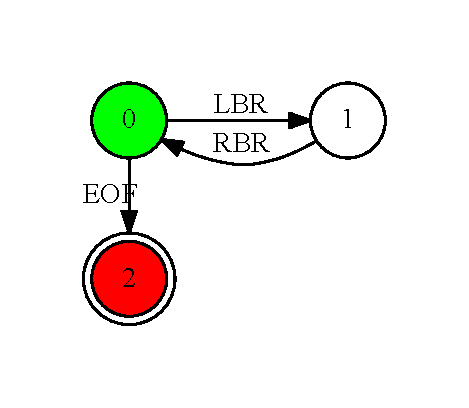
\includegraphics[width=2.5cm]{figures/in3.pdf}

            Грамматика:
            {\begin{align*}
                start& & &\Coloneq & &s \\
                s & & &\Coloneq & &\mbox{\texttt{LBR }} s \mbox{\texttt{ RBR }} s \\
                s & & &\Coloneq & &\varepsilon
            \end{align*}}
        \end{column}
        %\hspace{1cm}
        \begin{column}[T]{.6\textwidth}
            \vspace{-2em}
            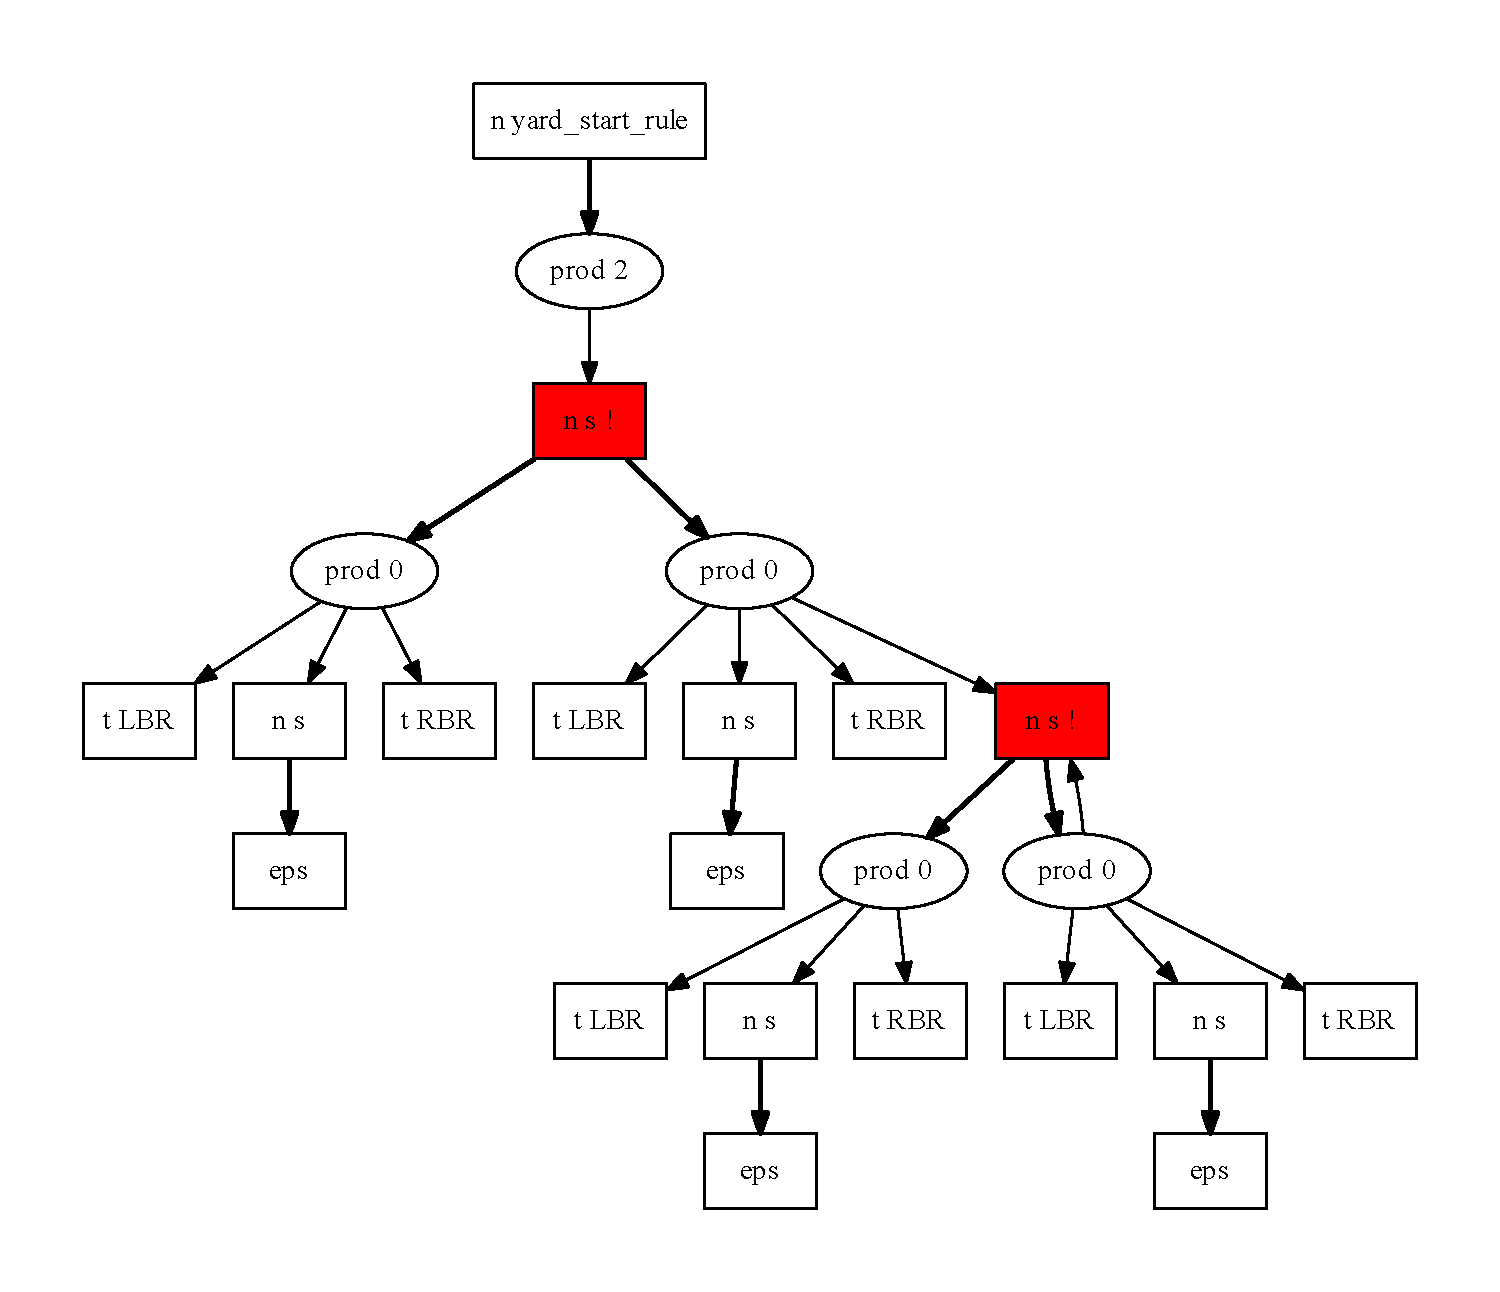
\includegraphics[width=1\textwidth]{figures/out3.pdf}
        \end{column}
    \end{columns}
\end{frame}

\begin{frame}
    \frametitle{Доказательство корректности алгоритма}
    {\small Формулировки утверждений. Идеи доказательств проговариваются устно.}
    \begin{rutheorem}[Пифагора: геометрическая формулировка]
        В прямоугольном треугольнике площадь квадрата, построенного на гипотенузе, равна сумме площадей квадратов, построенных на катетах.
    \end{rutheorem}

    \begin{rutheorem}[Пифагора: алгебраическая формулировка]
        В прямоугольном треугольнике квадрат длины гипотенузы равен сумме квадратов длин катетов.

        То есть, если обозначить длину гипотенузы треугольника через $c$, а длины катетов
        через $a$ и $b$, получим верное равенство: $a^2 + b^2 = c^2$.
    \end{rutheorem}

    \begin{rutheorem}[Обратная теорема Пифагора]
        Для всякой тройки положительных чисел $a$, $b$ и $c$, такой, что $a^2 + b^2 = c^2$, существует прямоугольный треугольник с катетами $a$ и $b$ и гипотенузой $c$.
    \end{rutheorem}
\end{frame}

\begin{frame}
    \frametitle{Архитектура решения}
    \begin{itemize}
        \item В реализации интересны архитектура, библиотеки, инструменты
        \item Не надо добавлять на слайд примеры кода
        \item Текст в квадратиках должен быть читаемым (крупным, а не как тут)
    \end{itemize}
    \begin{center}
        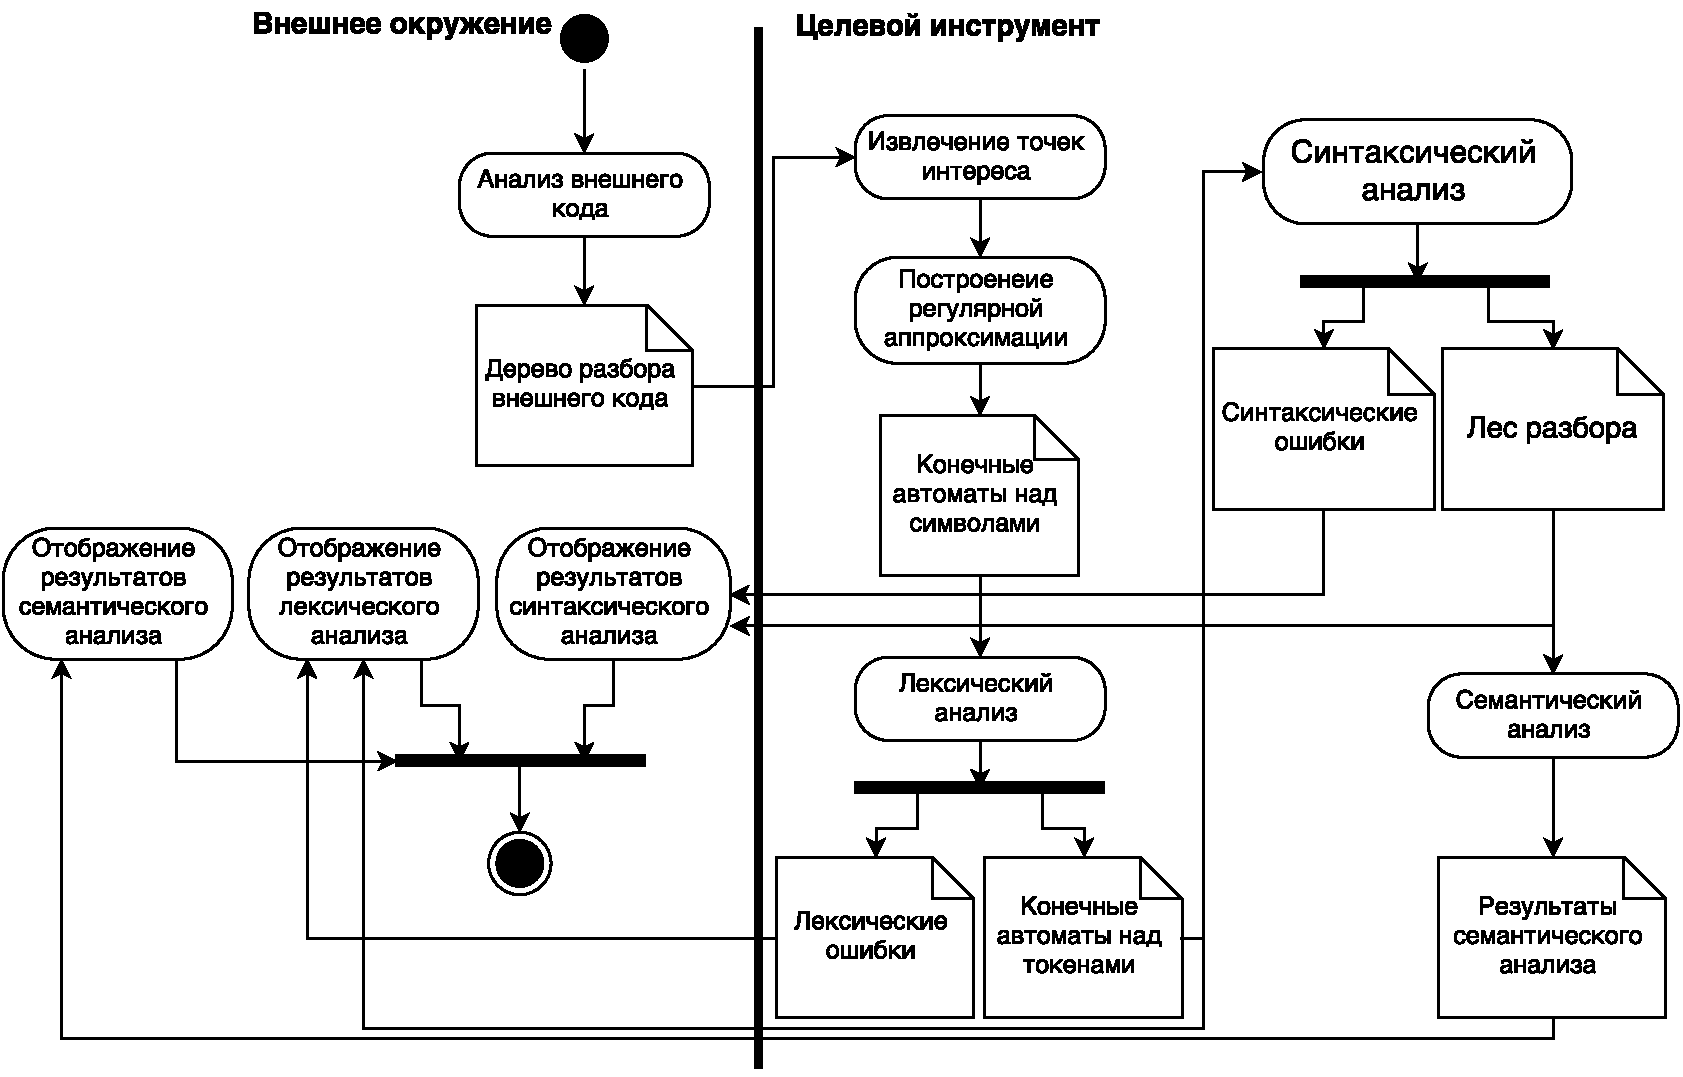
\includegraphics[width=0.7\textwidth]{figures/Activ_SEL_Processing.pdf}
    \end{center}
\end{frame}

\begin{frame}[t]
    \frametitle{Экспериментальное исследование}
    Постановка эксперимента
    \begin{itemize}
        \item На каком наборе данных проводилось экспериментальное исследование, почему были выбраны именно эти данные
        \item На каком оборудовании проводилось исследование
        \item Какие решения были выбраны для сравнения и почему
    \end{itemize}
\end{frame}

\begin{frame}[t]
    \frametitle{Результаты экспериментального исследования}
    \begin{itemize}
        \item Какие результаты показало экспериментальное исследование
        \item Желательно привести графики, иллюстрирующие полученные результаты
              \begin{itemize}
                  \item У иллюстраций должны быть подписи, у графиков~--- легенда, подписи к осям, например:
              \end{itemize}
    \end{itemize}
    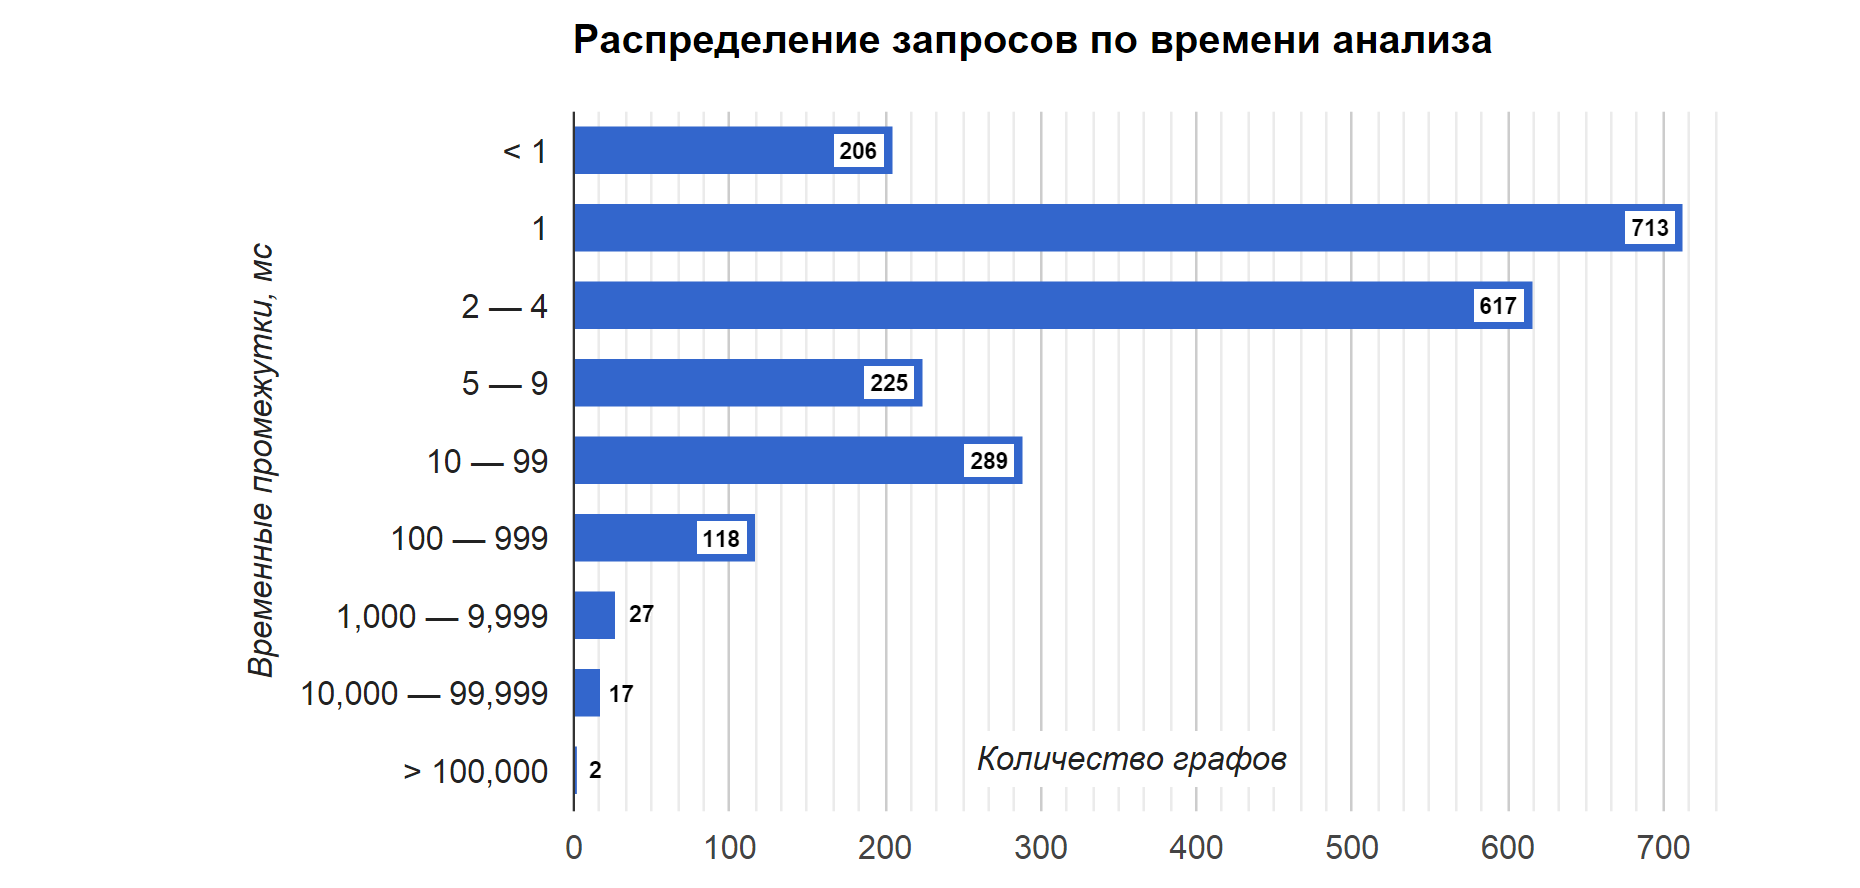
\includegraphics[width=13cm]{figures/dist.png}
\end{frame}

\begin{frame}
    \frametitle{Результаты}
    \begin{itemize}
        \item Практически то же, что и на слайде с постановкой задачи, но в совершенной форме~--- что делал лично автор
        \item Четкое отделение результатов своей работы (особенно для коллективных работ)
        \item Формулировать глаголами совершенного вида в прошедшем времени (\enquote{сделано}, \enquote{получено})
        \item Обсуждение (ограничения, валидность, альтернативы)
        \item Не нужно слайдов типа \enquote{Все}, \enquote{Вопросы?}, \enquote{Спасибо за внимание}
    \end{itemize}

    \begin{itemize}
        \item Если результаты были представлены на конференции и опубликованы, это желательно указать
    \end{itemize}
\end{frame}

%\addtocounter{framenumber}{1}
\appendix

\begin{frame}
    \frametitle{Дополнительный слайд}
    Например, с огромной страшной формулой всего, которая нужна для пояснения деталей при ответе на частый вопрос

    \begin{align*}
        \MoveEqLeft \lim_{\bigtriangleup t \to 0^+}\int_{\bigtriangleup t}^{T} \! \int_{\Omega} \! D(t_1,x) \frac{\varphi(t_1-\bigtriangleup t,x)-\varphi(t_1,x)}{(-\bigtriangleup t)} \, \mathrm{d}x \, \mathrm{d}t_1 \\
        &= \lim_{\bigtriangleup t \to 0^+} \int_{0}^{T} \! \int_{\Omega} \! D(t_1,x) \frac{\varphi(t_1-\bigtriangleup t,x)-\varphi(t_1,x)}{(-\bigtriangleup t)} \chi_{(\bigtriangleup t,T)}(t_1) \, \mathrm{d}x \, \mathrm{d}t_1 \\
        &=\int_{0}^{T} \! \int_{\Omega} \! D(t_1,x) \frac{\partial \varphi}{\partial t_1} (t_1,x) \, \mathrm{d}x \, \mathrm{d}t_1
    \end{align*}
\end{frame}

\begin{frame}
    \frametitle{Второй дополнительный слайд}
    \begin{itemize}
        \item Много дополнительных слайдов не надо: 1--2~вполне достаточно в большинстве случаев
        \item Кроме формул здесь могут быть схемы, рисунки, таблицы и другие вспомогательные материалы
    \end{itemize}

\end{frame}

\end{document}
